\documentclass{article}

\usepackage{graphicx}
\usepackage{tikz}
\usepackage{tikzsymbols}
\usetikzlibrary{calc,patterns,shapes.geometric}
\pagestyle{empty}
\usepackage[margin=0pt]{geometry}
\geometry{papersize={14in,12in}}

\def\centerarc[#1](#2)(#3:#4:#5){\draw[#1] ($(#2)+({#5*cos(#3)},{#5*sin(#3)})$) arc (#3:#4:#5);}

\begin{document}
	\begin{figure}
		\centering
		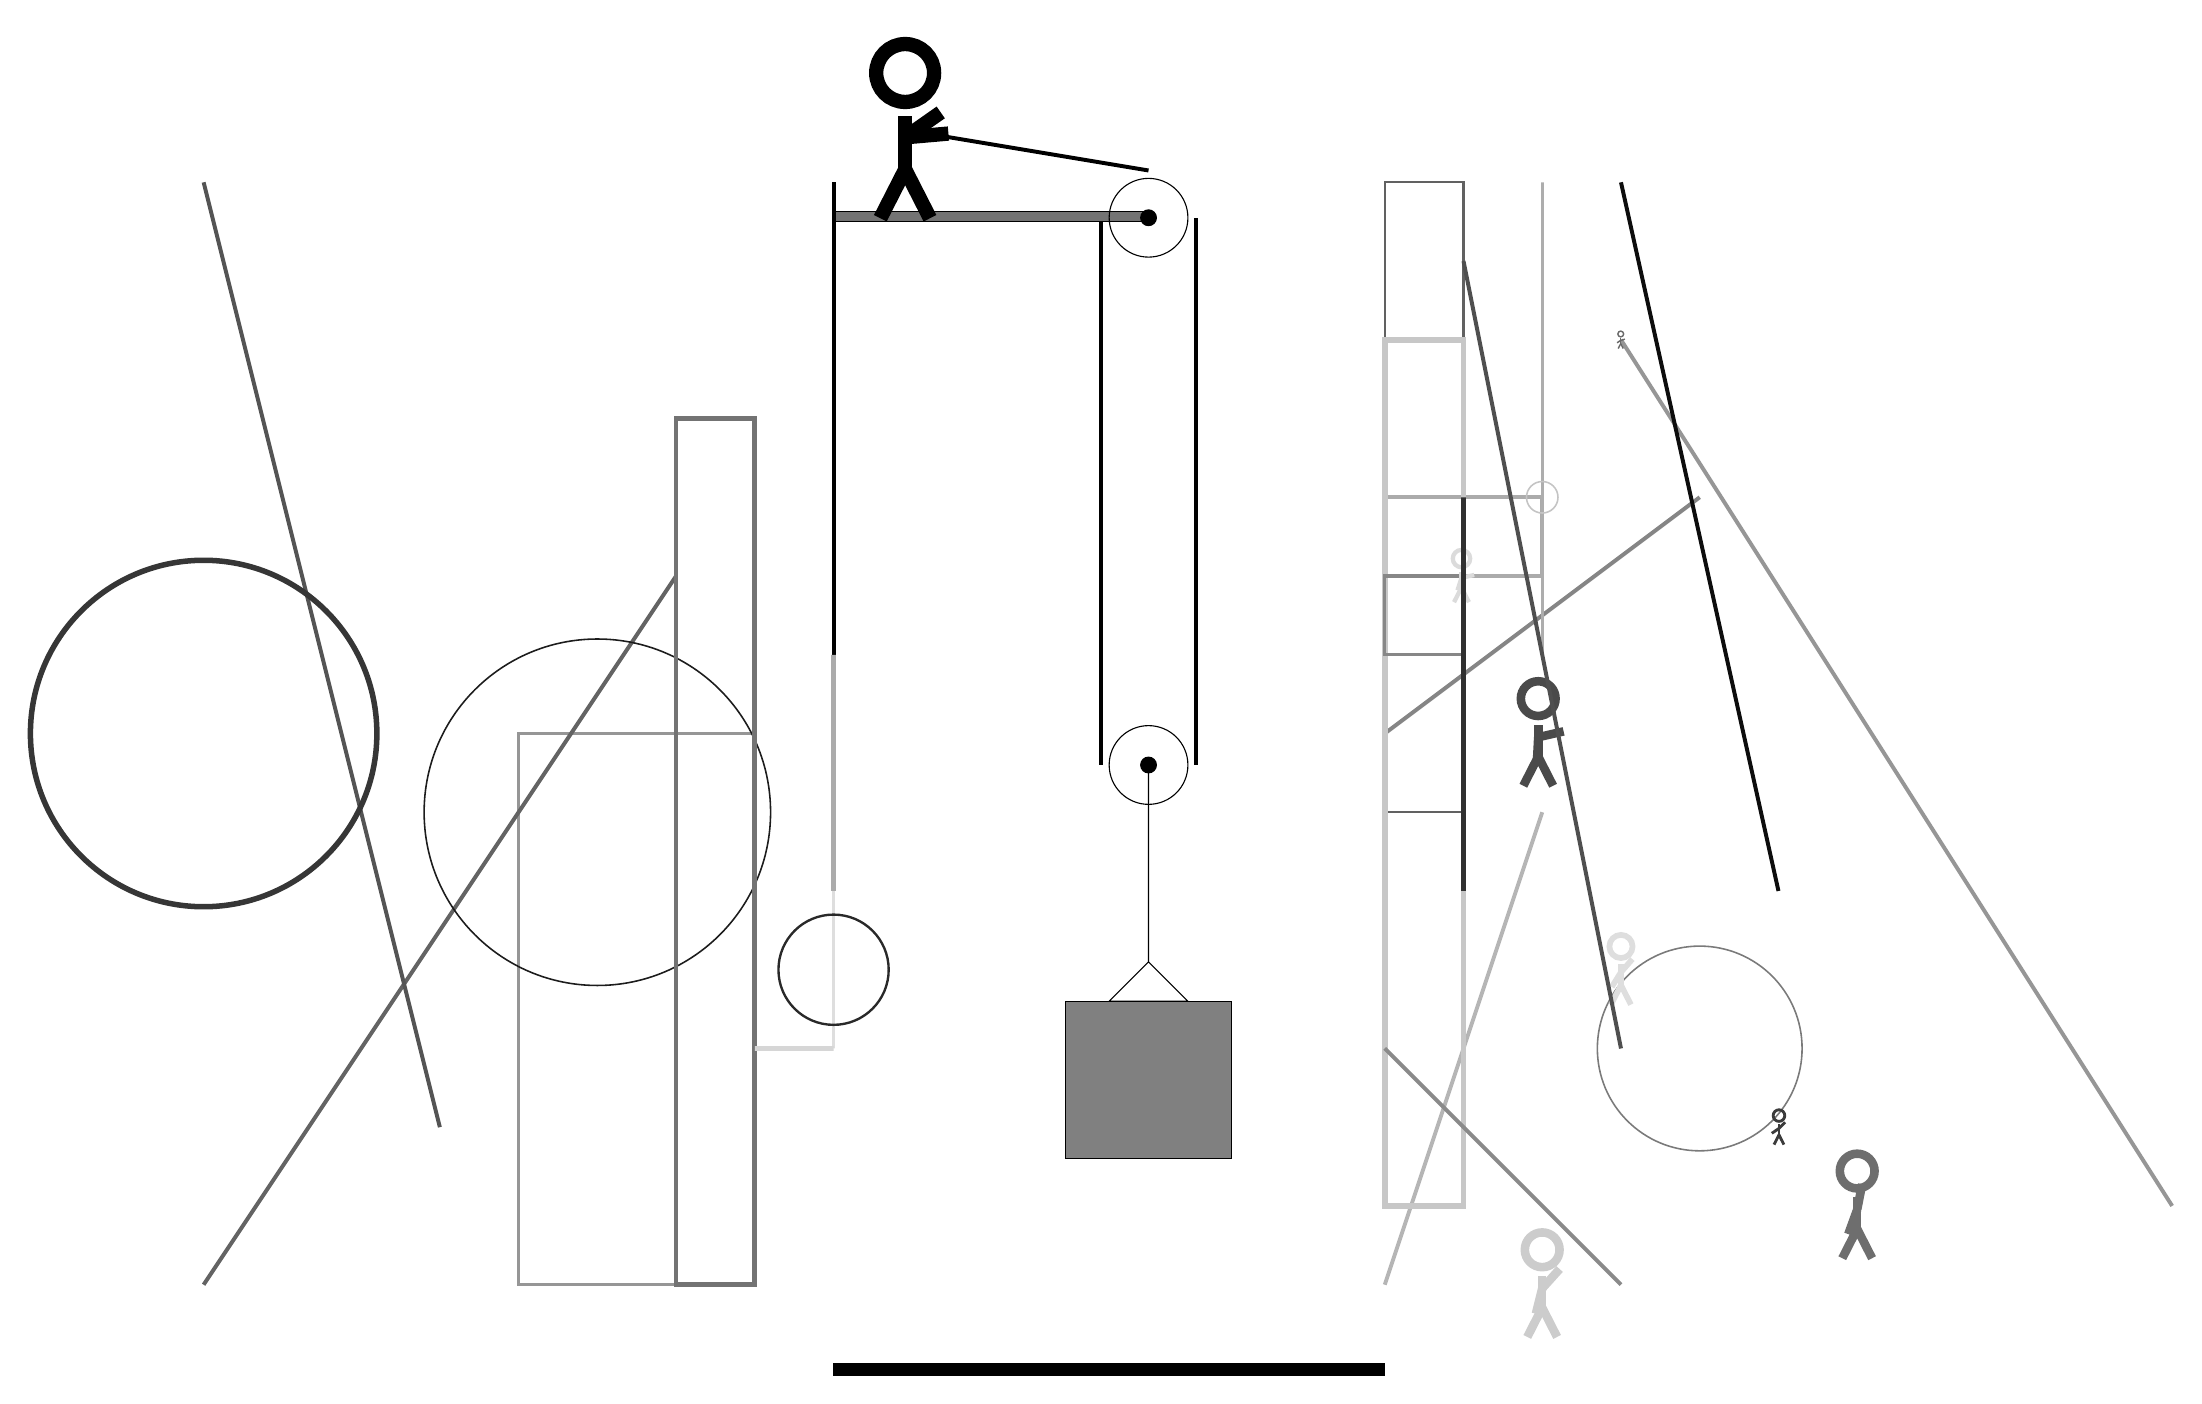
\begin{tikzpicture}
			%%%%% START %%%%%
			
			\draw[fill=black!55] (-2, 11.5) rectangle (2, 11.625);
			
			\draw (2, 4.6) circle (0.5);
			\draw[fill=black] (2, 4.6) circle (0.1);
			
			\draw (2, 11.55) circle (0.5);
			\draw[fill=black] (2, 11.55) circle (0.1);
			
			\node[line width=0.4mm, color=black!71] at (7, 5) {\Strichmaxerl[6][87][13]};
			
			\node[line width=0.5mm, color=black!20] at (7, -2) {\Strichmaxerl[6][76][48]};
			\draw[line width=0.4mm, color=black!41] (-3, 5) rectangle (-6, -2);
			\draw[line width=0.5mm, color=black!33] (5, 7) rectangle (7, 8);
			
			\draw[line width=0.3mm, color=black!62] (6, 4) rectangle (5, 12);
			\node[line width=0.4mm, color=black!57] at (11, -1) {\Strichmaxerl[6][70][79]};
			\draw [line width=0.2mm, color=black!52](9, 1) circle (1.3);
			\draw[line width=0.5mm, color=black!48](5, 5) -- (9, 8);
			\draw[line width=0.4mm, color=black!32] (7, 6) rectangle (7, 12);
			\draw[line width=0.4mm, color=black!13] (-2, 11) rectangle (-2, 1);
			\draw [line width=0.2mm, color=black!39](10, 2) circle (0.0);
			
			\draw[line width=0.5mm, color=black!29](7, 4) -- (5, -2);
			\draw[line width=0.7mm, color=black!22] (6, 10) rectangle (5, -1);
			
			\draw[line width=0.4mm, color=black!47] (5, 7) rectangle (6, 6);
			\node[line width=0.7mm, color=black!77] at (10, 0) {\Strichmaxerl[2][34][45]};
			\draw[line width=0.5mm, color=black!41](8, 10) -- (15, -1);
			
			\draw[line width=0.5mm, color=black!61](-4, 7) -- (-10, -2);
			\node[line width=0.5mm, color=black!13] at (8, 2) {\Strichmaxerl[4][58][49]};
			\draw[line width=0.5mm, color=black!69](6, 11) -- (8, 1);
			
			\draw [line width=0.2mm, color=black!89](-5, 4) circle (2.2);
			\draw[line width=0.6mm, color=black!55] (-3, -2) rectangle (-4, 9);
			\draw[line width=0.5mm, color=black!100](-2, 12) -- (-2, 3);
			\draw[line width=0.7mm, color=black!16] (-3, 1) rectangle (-2, 1);
			\draw[line width=0.5mm, color=black!67](-7, 0) -- (-10, 12);
			\node[line width=0.4mm, color=black!14] at (6, 7) {\Strichmaxerl[3][72][13]};
			\node[line width=0.6mm, color=black!59] at (8, 10) {\Strichmaxerl[1][32][17]};
			\draw[line width=0.6mm, color=black!81] (6, 8) rectangle (6, 3);
			\draw[line width=0.5mm, color=black!46](8, -2) -- (5, 1);
			\draw[line width=0.5mm, color=black!95](10, 3) -- (8, 12);
			\draw [line width=0.2mm, color=black!23](7, 8) circle (0.2);
			\draw [line width=0.3mm, color=black!84](-2, 2) circle (0.7);
			
			\draw [line width=0.7mm, color=black!79](-10, 5) circle (2.2);
			\draw[line width=0.7mm, color=black!33] (-2, 3) rectangle (-2, 6);
			
			\draw (2, 4.6) -- (2, 2.1) -- (1.5, 1.6) -- (2.5, 1.6) -- (2, 2.1);
			\draw[fill=black!50] (0.95, 1.6) rectangle (3.05, -0.4);
			
			\draw[line width=0.5mm] (1.4, 11.5) -- (1.4, 4.6);
			\centerarc[line width=0.5mm](2, 4.6)(180:360:0.6);
			\draw[line width=0.5mm](2.6, 4.6) -- (2.6, 11.55);
			\centerarc[line width=0.5mm](2, 11.55)(0:90:0.6);
			\draw[line width=0.5mm](2, 12.15) -- (-1, 12.65);
			
			\node at (-1, 12.65) {\Strichmaxerl[10][-175][35]};
			
			\draw[fill=black] (-2, -3) rectangle (5, -3.15);
			
			%%%%% END %%%%%
		\end{tikzpicture}
	\end{figure}	
\end{document}